\documentclass[tikz]{standalone}
\usetikzlibrary{calc}
\usepackage{mathrsfs}
\begin{document}
	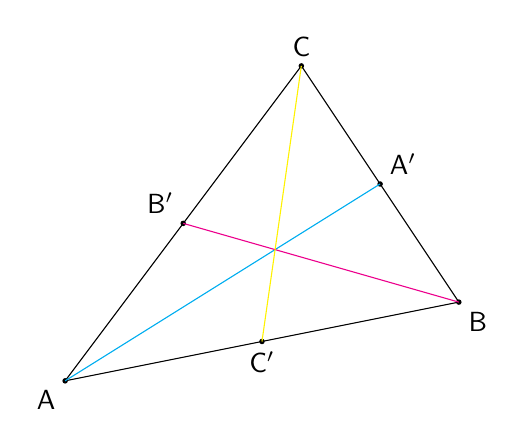
\begin{tikzpicture}
	\coordinate[label= below left:$\mathsf{A}$] (A) at (-1,2);
	\coordinate[label= below right:$\mathsf{B}$] (B) at (4,3);
	\coordinate[label= above:$\mathsf{C}$] (C) at (2,6);
	\draw (A) -- (B) -- (C) -- (A) -- cycle;
	\fill (A) circle (1pt);
	\fill (B) circle (1pt);
	\fill (C) circle (1pt);
	\coordinate[label= above right:$\mathsf{A^{\prime}}$] (Aprime) at ($(B)!0.5!(C)$);
	\fill (Aprime) circle (1pt);
	\coordinate[label= above left:$\mathsf{B^{\prime}}$] (Bprime) at ($(A)!0.5!(C)$);
	\fill (Bprime) circle (1pt);
	\coordinate[label= below:$\mathsf{C^{\prime}}$] (Cprime) at ($(A)!0.5!(B)$);
	\fill (Cprime) circle (1pt);
	\draw[cyan] (A) -- (Aprime);
	\draw[magenta] (B) -- (Bprime);
	\draw[yellow] (C) -- (Cprime);
	\end{tikzpicture}
\end{document}